\documentclass[fleqn]{template}
\usepackage[english]{babel}
\usepackage{underscore}

% packages andrea used, prob. delete
%\usepackage{float}                                                              
%\usepackage{booktabs}                                                           
%\usepackage{footnotes}                                                          
%\usepackage{graphicx}  


\setlength{\columnsep}{0.55cm}
% Distance between the two columns of text
\setlength{\fboxrule}{0.75pt}
% Width of the border around the abstract
\definecolor{color1}{RGB}{88,116,143}
\definecolor{color2}{RGB}{0,20,20} 


\usepackage{hyperref} % Required for hyperlinks
\hypersetup{hidelinks,colorlinks,breaklinks=true,urlcolor=color2,citecolor=color1,linkcolor=color1,bookmarksopen=false,pdftitle={Title},pdfauthor={Author}}


\usepackage{tikz}
\usepackage{verbatim}
%\usepackage[active,tightpage]{preview}
%\PreviewEnvironment{tikzpicture}
%\setlength\PreviewBorder{10pt}%
\usetikzlibrary{arrows,shapes,positioning,shadows,trees}

\usepackage{listings}
%% json style
\lstset{
    string=[s]{"}{"},
    stringstyle=\color{color1},
    comment=[l]{:},
    breaklines=true,
    commentstyle=\color{color2},
}

\usepackage{balance}

\usepackage{subfig}
\usepackage[font=bf,skip=\baselineskip]{caption}


\newcommand{\sd}[1]{\textbf{\color{olive}/* #1 (sd) */}}
\newcommand{\dd}[1]{\textbf{\color{red}/* #1 (dd) */}}
\newcommand{\wo}[1]{\textbf{\color{orange}/* #1 (wo) */}}
\newcommand{\kb}[1]{\textbf{\color{blue}/* #1 (kb) */}}
\newcommand{\az}[1]{\textbf{\color{blue}/* #1 (az) */}}



\begin{document}
    \JournalInfo{GESIS: KTSS} 

% Additional notes (e.g. copyright, DOI, review/research article)
\Archive{Technical Documentation}

\PaperTitle{Rich Context Competition Phase 2 (RCC-05)}

\Authors{Wolfgang Otto\textsuperscript{1}*,
         Andrea Zielinski\textsuperscript{1},
         Behnam Ghavimi\textsuperscript{1},
         Dimitar Dimitrov\textsuperscript{1},
         Narges~Tavakolpoursaleh\textsuperscript{1}
        }%kata: heisst der gute Mann nicht Behnam? ;)

\affiliation{\textsuperscript{1}\textit{Knowledge Technologies in the Social Sciences, GESIS -- Leibniz Institute for the Social Sciences, Cologne, Germany}} % Author affiliation

\affiliation{*\textbf{Corresponding author}: wolfgang.otto@gesis.org} % Corresponding author

% Keywords - if you don't want any simply remove all the text between the curly brackets
\Keywords{Dataset Mention Extraction --- Dataset Linking --- Research Method Extraction ---  Research Field Classification} 
 % Defines the keywords heading name
\newcommand{\keywordname}{Keywords}

\Abstract{This document describes the approach, results, and software submitted by team RCC-05 to the Rich Context Competition (RCC).
The team consists of members of the department \emph{Knowledge Technologies in the Social Sciences} of \emph{GESIS - Leibniz Institute for the Social Sciences} The goal of the RCC is to automatically discover and link research datasets, methods, and fields in social science publications. 
%The team was selected as one of four out of 19 participants in the first Phase of the competition to attend to the second Phase.
%This document describe the result of the work for both phases.
}

% create front
\flushbottom % Makes all text pages the same height
\maketitle % Print the title and abstract box
\thispagestyle{empty} % Removes page numbering from the first page


    
    %\input{sections/1-0-non-technical-overview}
    %\input{sections/2-0-litereature-review}
    %\input{sections/3-0-what-did-you}
    %\input{sections/4-0-what-worked-what-not}
    %\input{sections/5-0-summery-of-results-and-caveats}
    %\input{sections/6-0-lessons-learned-and-what-would-you-do-differently}
    %\input{sections/7-0-what-comes-next}
    %\input{sections/appendix}
    %\input{sections/8-0-description-of-code-and-documentation}
    
    \section{Introduction}
%\addcontentsline{toc}{section}{Introduction}
Scientists and analysts often face the problem of finding interesting research datasets and identifying who else used the data, in which research fields, and how the data has been analyzed from a methodological perspective.
To address these problems, the Coleridge Initiative organized the Rich Context Competition\footnote{\url{https://coleridgeinitiative.org/richcontextcompetition}}(RCC).
The competition invited international research teams to develop text analysis and machine learning tools that can discover relationships between research datasets, methods, and fields in scientific literature.
The competition took place between October 2018 and February 2019 and included two phases\footnote{\url{https://coleridgeinitiative.org/richcontextcompetition\#competitionschedule}}. The first phase was open for all teams which have submitted a letter of intent.
Teams are then provided with a corpus of social science publications to develop and train machine learning algorithms for automatic research dataset, methods and field detection and linking. 
More concretely, one major subtask consisted of linking dataset mentions to a given set of around 10,000 dataset descriptions from the ICPSR’s research data index.\footnote{\url{https://www.icpsr.umich.edu/index.html}}
Only the best four teams from the first phase are invited to the second phase of the competition and asked to discover research datasets, methods, and fields in a larger corpus of social science publications. All submitted algorithms have to be made publicly available as open source tools. With this document, we (team RCC-5) aim to fulfill another requirement, i.e., the documentation and summary of the developed approach including data pre-processing, algorithms, and software. 
%More about the type of scientific publications can be found in Section~\ref{subsec:rcc-corpus}.

%The Rich Context Competition\footnote{\url{https://coleridgeinitiative.org/richcontextcompetition}}(RCC) is organized by the Coleridge Initiative and targets both US and international researchers. The main goal of the competition is to automate the discovery of research datasets and the associated research methods and fields in social science publications. 
%task is to extract information from full texts to be able to create a network of publications, datasets and research methods.

%\subsection{Task Definition of the RCC}
%In both competition phases the task was to submit a software package which is able to process PDF (respectively extracted raw text) on the Servers of the organizers.
%The software have to be able to extract dataset mentions, research methods and research fields from the given publication. More about the type of scientific publications can be found in Section~\ref{subsec:rcc-corpus}.
%In the first phase additional the software has to be able to link dataset mentions to a given set of around 10,000 dataset descriptions originate from ICPSR\footnote{\url{https://www.icpsr.umich.edu/icpsrweb/ICPSR/}} research data index.

\subsection{General Approach and Software Components}
%\subsection{Our Approach on a technical perspective}
One of the central tasks in the RCC is the extraction of dataset mentions from text. 
Nevertheless, we considered the methods and fields discovery equally important.
To this end, we decided to follow a module-based approach and developed tools that can be used separately but also as parts of a data processing pipeline.
Figure~\ref{figure:pipeline} shows an overview of the software modules developed for the RCC competition, including their dependencies. Here, the upper three modules (gray) describe the pre-processing steps (cf. Section~\ref{sec:prepro}).
The lower four modules (blue) are used to generate the output in a pre-specified format. 
The pre-processing step consists of extracting metadata and pure text from PDF documents. The extraction itself is done using the Cermine Tool\footnote{\url{https://github.com/CeON/CERMINE}} which returns a Journal Article Tag Suite\footnote{\url{https://jats.nlm.nih.gov}}(Jats) XML document. Then, in a second step,
text, metadata and references are extracted. The output of the pre-processing is then used by the software modules responsible for tackling the individual sub-tasks, i.e., discovering research datasets (cf. Section~\ref{sec:dataset-extraction}), methods (cf. Section~\ref{section:research_method_extraction}) and fields (cf. Section~\ref{section:field_classification}). Section~\ref{sec:techdoc} provides the technical details of the modules, i.e., input, output, and how to run the modules. 


%After pre-processing, a Named Enity Recognition module is used to find data set mentions. The training corpus and process is described in Section~\ref{sec:dataset-extraction}.

%In the next step, we combine all recognized mentions for each publication and compare these mentions to the metadata from `data_sets.json`.
%The mentions are used in an interim format which also persists the sentence of each mention. Also, all years are extracted from theses sentences
%and used in the retrieval process. After retrieving the best matching results, theses are returned in the target format for `data_set_citation.json`.

%For identifying research fields, we trained a classifier on abstracts and metadata crawled from the Social Science Open Access Repository\footnote{\url{https://www.ssoar.info}} (SSOAR). We used the OAI-API for this and the crawler is delivered in the module.
%We tried different classifiers and selected the best performing one, a [fasttext]() classifier, i.e. a neural net based approach with a high performance.



\begin{figure}[t]
    \centering
    \resizebox{!}{7cm}{\tikzset{
  basic/.style  = {draw, text width=2cm, drop shadow, font=\sffamily, rectangle},
  root/.style   = {basic, rounded corners=2pt, thin, align=center,
                   fill=color1!30},
  level empty/.style={},
  level 1/.style={sibling distance=2mm},
  level 2/.style = {basic, rounded corners=4pt, thin, align=center, fill=color1!60},
  level 3/.style = {basic, rounded corners=2pt, thin,
                    align=center, fill=color2!10, text width=6.5em}
}


\begin{tikzpicture}[
  node distance=1.7cm and 1.7cm,
  edge from parent/.style={->,draw},
  >=latex
  ]

% root of the the initial tree, level 1
%\node[root] {RCC-05 Pipeline Components}
% The first level, as children of the initial tree
%  child {node[level 2] (c1) {Preprocessing}}
%  child {node[level 2] (c2) {Dataset Linking}}
%  child {node[level 2] (c3) {Research Method Extraction}}
%  child {node[level 2] (c4) {Research Field Classification}};

% The second level, relatively positioned nodes
\begin{scope}[every node/.style={level 3}]
    \node [] (c11) {PDF to Jats XML};
    \node [below of = c11] (c12) {Metadata Extraction from Jats XML};
    \node [right = 0.4cm of c12] (c13) {Jats XML to paragraphs in JSON};
\end{scope}

\node [level 2, below = 1.5cm of c13, xshift=0pt] (c21) {Extract Dataset Mentions};
\node [level 2, below =  0.5cm of c21] (c22) {Link Mention to Dataset List (optional)};
\node [level 2, below = 1.5cm of c13, xshift=3cm]  (c31) {Extract Research Methods};
\node [level 2, below = 1.5cm of c12, xshift=0pt] (c41) {Predict Research Fields};

\node [level empty, below = 2.7cm of c21] (c51){};
 



% lines from each level 1 node to every one of its "children"
%\foreach \value in {1,...,3}
%  \draw[->] (c1.195) |- (c1\value.west);
%\draw[->] (c1.south) -| (c11.north);
\draw[->] (c11.south) -| (c12.north);
\draw[->] (c11.east)  -- +(1,0) -| (c13.north);

\draw[->] (c13.south) -| (c21.north);
\draw[->] (c21.south) -| (c22.north);

\draw[->] (c13.east) -- +(1.7,0) -| (c31.north);

\draw[->] (c12.south) -| (c41.north);

%\foreach \value in {1,...,1}
%  \draw[->] (c3.195) |- (c3\value.west);
\end{tikzpicture}

\begin{comment}
    Old Pipeline (4 Elements)
    \node[level 2] (c1) {(1) Preprocessing};
    \node[level 2, right= 3cm of c1] (c2) {(2) Dataset Linking};
    \node[level 2, right= of c2] (c3) {(3) Research Method Extraction};
    \node[level 2, right= of c3] (c4) {(4) Research Field Classification};
    \draw[->] (c1) |- (c2);
    \draw[->] (c1.30) -- +(0,0.7) -| (c3.north);
    \draw[->] (c1.150) -- +(0,1.3) -| (c4.north);

\end{comment}
}
    \caption{Software modules. The figure shows an overview of the individual software modules described in this document and their dependencies. Modules colored in gray represent our pre-processing pipeline, whereas blue-colored modules represent the three main tasks of the RCC.}
    \label{figure:pipeline}
\end{figure}

\subsection{First Phase Feedback}
After the first phase, each team received feedback from the organizers of the RCC.
The feedback is twofold and consists of a quantitative and qualitative evaluation. Unfortunately, our team did not perform very well regarding precision and recall. In contrast to this, our approach has been found convincing regarding the quality of results. The qualitative feedback result from a random sample of ten documents that are given to four judges.
Judges are then asked to manually extract dataset mentions and calculate the overlap between their dataset extractions and the output of our algorithm.
Other factors that judges took into consideration are specificity, uniqueness and multiple occurrences of dataset mentions.
As for the extraction of research methods and fields no ground truth has been provided, these tasks were evaluated against the judges' expert knowledge.
Similarly to the extraction of dataset mentions, specificity and uniqueness have been considered for these two tasks.
The feedback our team received acknowledged the fact that no ground truth has been provided and our efforts regarding the extraction of research methods and fields.
%Feedback by RCC
%Section~\ref{} gives detailed overview of data provided by the RCC and additional data sources used in our approach. 


    \section{Data and Pre-processing}
This section describes the data provided by the organizers of the RCC, the external data sources we used as well as our pre-processing steps.
\subsection{The RCC Corpus}
\label{subsec:rcc-corpus}
For the first phase, the data provided by the organizers consisted of 5,000 publications. Additionally, a development fold of 100 plain text publications, their metadata, a list of datasets of interest (including all datasets that were explicitly referenced in the curated corpus) were given. The list of datasets should not be considered complete as  there could be additional datasets mentioned in these publications. 
The organizers also provided examples of social science research methods and fields vocabularies in term of SAGE Publications research field and method vocabularies. 
In the second phase of the competition, an additional set of 5,000 publications from the social sciences has been provided.
\subsection{External Data Sources}
For developing our algorithms, we also utilized two external data sources. For the discovery of research methods and fields, we resort to data from Social Science Open Access Repository\footnote{\url{https://www.gesis.org/ssoar/home}} (SSOAR). 
SSOAR is maintained at GESIS – Leibniz Institute for the Social Sciences collects and archives literature of relevance to the social sciences. In SSOAR, full texts are indexed using controlled social science vocabulary (Thesaurus\footnote{\url{https://www.gesis.org/en/services/research/tools/thesaurus-for-the-social-sciences}}, Classification\footnote{\url{https://www.gesis.org/angebot/recherchieren/tools-zur-recherche/klassifikation-sozialwissenschaften} (in German)}) and are assigned rich metadata. SSOAR offers documents in various languages. The corpus of English language publications that can be used for purposes of the competition consists of a total of 13,175 documents. All SSOAR documents can be accessed through the OAI-PMH\footnote{{\url{http://www.openarchives.org}}} interface. 
Another external source that we used for discovery of research methods is the ACL Anthology Reference Corpus~\cite{bird2008acl}. ACL ARC is a corpus of scholarly publications about computational linguistics.  
The corpus consists of a total of 22,878 articles.

%SSOAR contains 
%\subsubsection{SSOAR}
%\label{subsubsec:ssoar-dataset}
%Andrea: 
%Benam: 

%For example, 22,453 records with English abstracts in SSOAR also contain information about the classification of social sciences documents - 156 different labels of the classification.

%For items with English title and classoz classification, the numbers are different. SSOAR includes 15,522 items with English titles and cover 154 classoz classification labels.
%Classification Schemes used in the anntotations of SSOAR publications.
%\begin{enumerate}
%    \item Thesaurus Social Science (thesoz)
%    \item classification of the social sciences %(classoz)\footnote{\url{https://www.gesis.org/angebot/recherchieren/tools-zur-recherche/klassifikation-sozialwissenschaften} (in German)}
%    \item ddc classification (ddc)
%\end{enumerate}

%\subsubsection{ACL}
%ACL 

%\dd{table of external data/sources?SSOAR metedata including abstracts and classifications(thesoz/ classsoz)}

\subsection{Pre-processing}
\label{sec:prepro}
Although the organizers of the RCC, offered plain texts for the publication, we decided to build our own pre-process pipeline. The pipeline uses the Cermine Tool to extract information from PDF documents. The main benefit of using this tool is the structured metadata output including better disambiguation of sections and paragraphs in the publications. The output XML file uses the Journal Article Tag Suite\footnote{\url{https://jats.nlm.nih.gov}}. For the competition, there are only two interesting elements of the Jats XML format, i.e., $<$front$>$ and $<$body$>$. The $<$front$>$ element contains the metadata of the publication, whereas the $<$body$>$ contains the publication text. Another advantage of Cermine is that the hyphenation and segmentation of paragraphs are carried out automatically. 
As a last step of the pre-processing, we remove all linebreaks from the publication text and output a list of metadata fields and values as shown in Table~\ref{tab:example-paragraph} for each publication paragraph.

\begin{table}[h]
    \centering
     \caption{An Example output of our pre-processing for a paragraph in a given publication.}
    \begin{tabular}{ll}
        \toprule
        {} &                            Example Text Field Data\\
        \midrule
        publication\_id     &                                              12744 \\
        
        label              &              paragraph\_text \\
        text               &  A careful reading of text, word\\
                    & for word, was ... \\
        section\_title      &               Data Analysis \\
        annotations        &  [\{'start': 270, 'end': 295,\\
                           &        'type': 'bibref', ... \\
        
        section\_nr         &                                             [3, 2] \\

        text\_field\_nr      &                                                 31 \\
        para\_in\_section    &                                                  1 \\
        
        \bottomrule
    \end{tabular}
    \label{tab:example-paragraph}
\end{table}


    \section{Dataset Extraction}
\label{sec:dataset-extraction}
\subsection{Task Description}
In scientific literature, datasets are specified to indicate, e.g., the data on which a analysis is performed, a certain finding or a claim is based on. In this competition, we focus on (i) extracting and (ii) linking datasets mention from social science publications to a list of given dataset references.
Identifying dataset mention in literature is a challenging problem due to the lack of an established style of citing datasets.
Furthermore, in many research publication, a correct citation of datasets is entirely missing~\cite{boland2012identifying}. 
The following two sentences exemplify the problem.\\ 
\textbf{Example 1}: \emph{P-values are reported for the one-tail paired t-test on \emph{Allbus} (dataset mention) and \emph{ISSP} (dataset mention).}\\
\textbf{Example 2}: \emph{We used \emph{WHO data from 2001} (dataset mention) to estimate the spreading degree of AIDS in Uganda.}\\
We treat the problem of detecting dataset mentions in full-text as a Named Entity Recognition (NER) task. 

    %COMMENT (AZ): The following paragraph might be skipped
\paragraph{Formal problem definition}%\ \\[1pt]
%Let $D$ denote a set of existing datasets $d$. The Named Entity Recognition task is defined as the identification of dataset mentions $m$ in a sentence where $m$ references a dataset $d$. 
Let $D$ denote a set of existing datasets $d$ and the knowledgebase $K$ as a set of known dataset references $k$. Furthermore, each element of $K$ is referencing an existing dataset $d$. The Named Entity Recognition and linking task is defined as (i) the identification of dataset mentions $m$ in a sentence, where $m$ references a dataset $d$ and (ii) linking them, when possible, to one element in $K$ (i.e., the reference dataset list given by the RCC). 


\subsection{Challenges}
With our method, we focus on the extraction of dataset mentions in the body of the full-text of scientific publications. We recognize three types a dataset can be mentioned: (i) The full name of a dataset like ''National Health and Nutrition Examination Survey``, (ii) an abbreviation (''NHaNES``) or (iii) a vague reference, e.g., ''the monthly statistic``. 
By each of these varieties, the NER task faces particular challenges. For the first type, the used dataset name can vary in different publications. Where one publication cites the dataset with ''National Health and Nutrition Examination Survey`` the other could use the words  ''Health and Nutrition Survey``.
In a case where abbreviations are used a disambiguation problem occurs, e.g., in ''WHO data``. WHO may describe the World Health Organization or the White House Office.
The biggest challenge is again the lack of a precise gold standard that can be used to train a classifier.
%The major challenge of using a NER approach to detect dataset mentions in text is the necessity of an annotated training corpus which is not given by the RCC.
In the following we describe how we have dealt with this lack of ground truth data.  
\subsection{Phase one approach}
The challenge of missing ground truth data is the main problem to handle during this competition. To this end, supervised learning methods for dataset mentions extraction from text are not directly applicable. To overcome this limitation, we resort to the provided list of dataset mentions and publication pairs and re-annotate the particular sentences in the publication text. This re-annotation is then used to train Spacy's neural network based NER model\footnote{\url{spacy.io}}. We created a holdout set of 1000 publications and a training set of size 4000. We train our model using publication paragraphs as training samples. In the training set, 0.45 percent of the paragraphs contained mentions.  For each positive training example, we added a negative example that does not contain dataset mentions and is sampled at random.  
%(paragraphs without mentions: 265029; paragraphs with mentions: 12566)
%We extracted all paragraphs with mentions and merged them with a randomly chosen subset of paragraphs without mentions with the same the size resulting in 25132 paragraphs.
We used a batch size of 25 and a dropout rate of 0.4. The model was trained for 300 iterations.
\paragraph{Evaluation}
We evaluated our model with respect to four metrics: strict precision and recall, and partial precision and recall. While the former are standard evaluation metrics, the latter are their relaxed variants in which the degree to which dataset mentions have to match can vary. 
%This evaluation scheme is pased Semeval 2013 description can be found in this blog
% \url(http://www.davidsbatista.net/blog/2018/05/09/Named_Entity_Evaluation/)
%In the evaluation method, we have a parameter to control the weight of only partly matched mentions. 
Consider the following example of a partial match: "National Health and Nutrition Examination Survey" is the extracted dataset mention whereas, "National Health and Nutrition Examination Survey (NHANES)" represents the true dataset mention. 
%We set $alpha$ to $1.0$, meaning that the true and extracted dataset mention have to overlap in at least one token to count as a match. Setting $\alpha$
\begin{table}[b]
    \center 
    \caption{Results(phase one). } 
    \begin{tabular}{lc} 
        \toprule
        Metric  & Value \\
        \midrule
        Partial Precision   & 0.93 \\
        Partial Recall      & 0.95 \\
        \midrule
        Strict Precision    & 0.80 \\
        Strict Recall       & 0.81 \\ 
        \bottomrule \\ 
    \end{tabular} 
    \label{table:dataset-mention-eval} 
\end{table}
%Evaluation results of dataset mention extraction on holdout set

Table~\ref{table:dataset-mention-eval} show the results of the dataset mention extraction on the holdout set. The model is able to achieve high strict precision and recall values. As expected, the results are even better for the partial version of the metrics. But, this version indicates that even if we are not able to exactly match the dataset mention in text, we can find the right context with very high precision at least.
%Notably  The results show, that in 10\% of the found matches we have not found the strict correct dataset mention, but the correct position and there is a partial match.

\subsection{Phase two approach}
In the second phase of the competition additional 5,000 publications have been provided. We extended our approach to consider the list with dataset names supplied by the organizers and re-annotated the complete corpus of 15.000 publication in the same manner as in phase one to obtain training data. This time we split the data in 80\% for training and 20\% for test.   

\paragraph{Evaluation}
We resort to the same evaluation metrics as in phase one. However, we calculate precision and recall on the full-text of the publication and not on the paragraphs as in the first phase. Table~\ref{table:dataset-mention-eval-phase-two} show the results achieved by our model. We observe a lower precision and recall values. Compared to phase one, there is also a smaller difference between the precision an recall values for the strict and partial version of the metrics. 
\begin{table}[hb]
    \center 
    \caption{Results(phase two).} 
    \begin{tabular}{lc} 
        \toprule
        Metric  & Value \\
        \midrule
        Partial Precision   & 0.51 \\
        Partial Recall      & 0.90 \\
        \midrule
        Strict Precision    & 0.49 \\
        Strict Recall       & 0.87 \\ 
        \bottomrule \\ 
    \end{tabular} 
    \label{table:dataset-mention-eval-phase-two} 
\end{table}


    \subsection{Research Method Extraction}
\label{section:research_method_extraction}
%\wo{Andrea ask for a structure. I suggest: Task (What to do), Challenges (Concrete Problem), Our Approach (Solution), Development of the controlled Vocabulary, Development of Training Corpus, Evaluation (if possible from Andreas introspection of SSOAR results, how good we solved the problem)}


\subsubsection{Task Description}
Inspired by a recent work of Nasar et al.
\cite{nasar2018information}, we define a list of basic entity types that give key-insights into scholarly publications. 
We adapted the list of semantic entity types to the domain of the social sciences with a focus on \textit{research methods},
but also including related entity types such as \textit{Theory, Model, Measurement, Tool, Performance}. We suspect that the division into semantic types might be helpful to find \textit{research methods}, because
related semantic entities types might provide clues or might be directly related to the research method itself.
For instance, in order to realize a certain research objective, an experiment is instrumented where a specific combination of \textit{methods} is applied to a \textit{data set} that might be intellectual or \textit{software}, thus achieving a specific \textit{performance} and result in that context.\\
%\\
\textbf{Example}: \textit{P-values} (measurement) are reported for the \textit{one-tail paired t-test} (method) on \textit{Allbus} (dataset) and \textit{ISSP} (dataset).\\


    %COMMENT (AZ): The following paragraph might be skipped
\paragraph{Formal problem definition}%\ \\[1pt]
Let $E$ denote a set of entities. The Named Entity Recognition and Linking task consists of (i) identifying entity mentions  $m$ in a sentence and, (ii) linking them, when possible, to a  reference knowledge base  $K$ (i.e, the SAGE Thesaurus\footnote{http://methods.sagepub.com}) 
and (iii) assigning a type to the entity, e.g., \textit{research method}, selected from a set of given types. 
Given a textual named entity mention $m$ along with the unstructured text in which it appears, the goal is to produce a mapping from the mention  $m$ to its referent real world entity  $e$ in  $K$.

\subsubsection{Challenges}
There are some major challenges that any named entity recognition, classification and linking system needs to handle.
First, regarding NER, identifying the entities boundary is important, thus detecting the exact sequence span. 
Second, ambiguity errors might arise in classification. For instance,`range' might be a domain-specific term from the knowledge base or belong to the general domain vocabulary. This is a challenging task for which context information is required. 
In the literature, this relates to the problem of \textbf{domain adaptation} which includes fine-tuning to specific named entity classes\footnote{apart from those used in traditional NER systems like \textit{Person}, \textit{Location}, or \textit{Organization} with abundant training data, as covered in the Stanford NER system\cite{finkel2005incorporating}}.
With respect to entity linking, another challenge is detecting name variations, since entities can be referred to in many different ways.
Semantically  similar words, synonyms or related words, which might be lexically or syntactically different, are often not listed in the knowledge base 
(e.g., the lack of certain terms like `questioning' but not `questionnaire').  This problem of automatically detecting these relationships is generally known as \textbf{linking problem}. 
Note that part of this problem also results from PDF-to-text conversion which is error-prone. 
Dealing with incomplete knowledge bases, i.e. \textbf{handling of out of vocabulary (OOV) items}, is also a major issue, since 
knowledge bases are often not exhaustive enough and do not cover specific terms or novel concepts from recent research.
Last but not least, the combination of different semantic types gives a more coherent picture of a research article. We hypothesize that such information would be helpful and results in an insightful co-occurrence statistics, and provides additional detail directly related to entity resolution, and finally helps to assess the \textbf{relevance of terms} by means of a score.

 
\subsubsection{Our Approach - Overview} 
Our context-aware framework builds on Stanford’s CoreNLP and Named Entity Recognition System\footnote{\url{https://nlp.stanford.edu/projects/project-ner.shtml}}. 
The information extraction process follows the workflow depicted in Figure~\ref{figure:pipeline}, using separate modules for pre-processing, classification, linking and term filtering.

We envision the task of finding entities in scientific publications as a sequence labeling problem, 
where each input word is classified as being of a dedicated semantic type or not.
In order to handle entities related to our domain, we train a novel machine learning classifier with major semantic classes,
%(see Table~\ref{tab:SemanticTypes}), 
using training material from the ACL RD-TEC 2.0 dataset  \cite{qasemizadeh2016acl}.
Apart from this, we follow a domain adaptation approach inspired by \cite{agerri2016robust} and ingest semantic background knowledge extracted from external scientific corpora, in particular the ACL Anthology~\cite{bird2008acl,gildea2018acl}.
We perform entity linking by means of a new gazetteer-based SAGE dictionary  of Social Research Methods  \cite{lewis2003sage}, thus putting a special emphasis on the social sciences. The linking component addresses the synonymy problem and matches an entity despite name variations such as spelling variations. 
Finally, term filtering is carried out based on a termhood and unithood, while scoring is achieved by calculating a relevance score based on TF-IDF (cf.  Section~\ref{para:relscore}).

%In order to conduct this study\dd{Study?}, 
Our research experiments are based on the repository for the Social Sciences SSOAR as well as the train and test data of the Rich Context Competition corpus\footnote{\url{https://coleridgeinitiative.org/richcontextcompetition}
with a total of 5,000 English documents}.
Our work extends previous work on this topic (cf. \cite{eckle2013automatically}) in various ways: First, we do not limit our study to abstracts, but use the entire fulltext. Second, we focus on a broader range of semantic classes, 
i.e. \textit{Research Method}, \textit{Research Theory}, \textit{Research Tool} and \textit{Research Measurement}, tackling also the problem of identifying novel entities.
 

\begin{figure}
\label{pipeline}
  \centering
    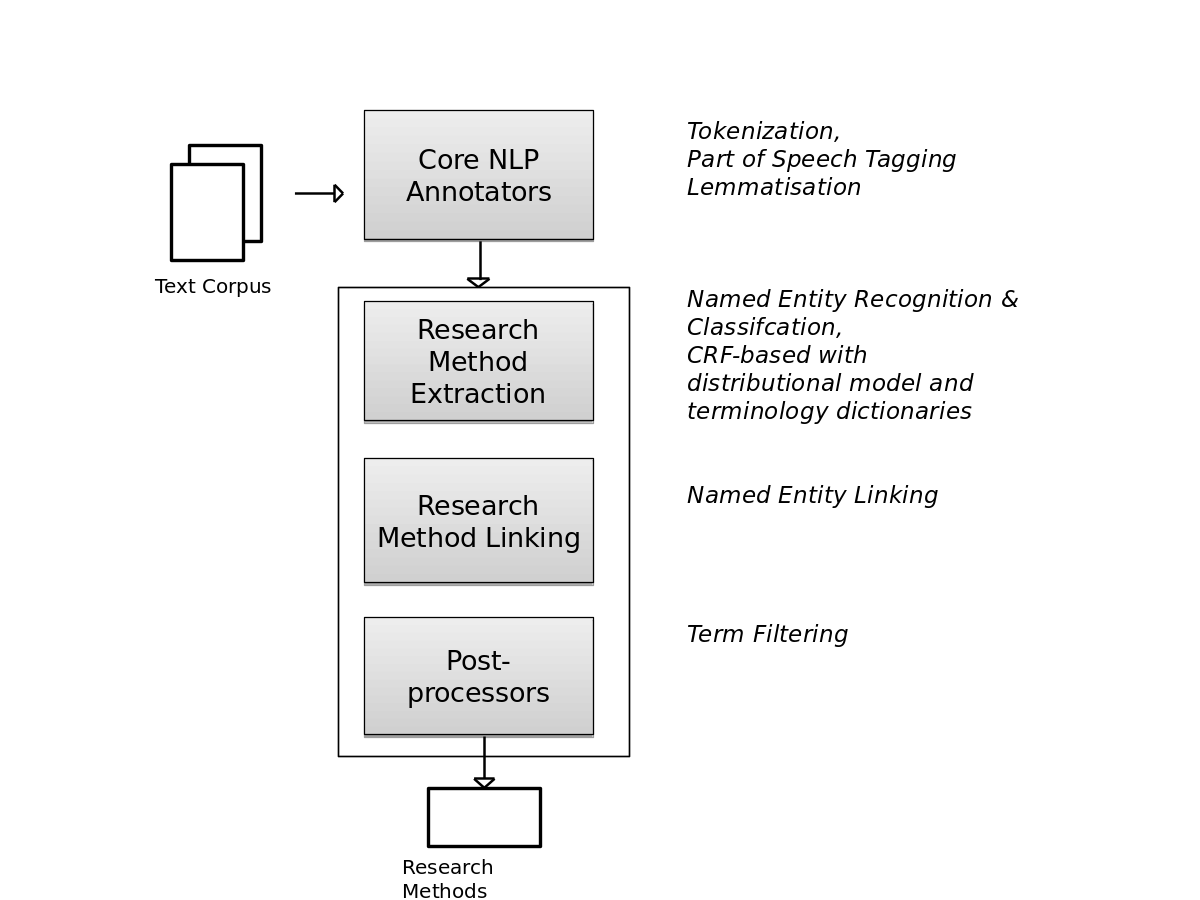
\includegraphics[width=0.47\textwidth]{figures/research-methods/pipeline.png}
    \caption{Overview of the entity extraction pipeline}
\end{figure}

\paragraph{Distributed Semantic Models}%\ \\[1pt]
\label{subsec:dist-model}
For domain adaptation, we integrate further background knowledge. We use vector embeddings  of words trained on additional corpora and which serve as input features to the CRF model. Semantic representations of words are a successful extension of common features, resulting in higher NER performance~\cite{Turian} and can be trained offline.


In this work, the word vectors were learned  from the scientific ACL ARC\footnote{\url{https://acl-arc.comp.nus.edu.sg/}} using Gensim with the skip gram model (cf. \cite{mikolov2013distributed}) 
and a pre-clustering algorithm\footnote{
Word embeddings are trained with a skip gram model using embedding size equal to 100, word window equal to 5, minimal occurrences of a word to be considered 10. Word embeddings are clustered using agglomerative clustering with a number of clusters set to {500,600,700} Ward linkage with euclidean distance is used to minimize the variance within the clusters.}. A summary of the size of the unlabeled  English data used for training word embeddings can be found in Table~\ref{tab:UnlabeledData}.

\begin{table}
\center
\small
  \caption{English data used for Training Word Embeddings}
  \label{tab:UnlabeledData}
  \begin{tabular}{lll}
    \toprule
    Corpus & Articles &  Documents/Tokens  \\
    \midrule
   ACL Corpus
    %ACL Anthology Reference Corpus
    &  22,878  &  806,791/2.5 GB \\ 
  \bottomrule
\end{tabular}
\end{table}

\paragraph{Features}%\ \\[1pt]
The  features incorporated into the linear chain CRF are shown in the Table~\ref{tab:features}. The features depend mainly on the observations  and  on  pairs  of  adjacent  labels, using a log-linear  combination. However, since simple token level training of CRFs leads to poor performance, more effective text features such as word shape, orthographic, gazetteer, Part-Of-Speech (POS) tags, along with word clustering (see Section~\ref{subsec:dist-model}) have been used.
%
\begin{table}
\small
  \caption{Features used for NER}
  \label{tab:features}
  \center
  \begin{tabular}{lc}
    \toprule
  \textbf{Type} &  \textbf{Features} \\
    \midrule
\textbf{Token unigrams} 	   &    $w_{i-2}$, $w_{i-1}$, $w_{i}$, $w_{i+1}$, $w_{i+2}$, ... \\

\textbf{POS unigrams} 	   &    $p_{i}$, $p_{i-1}$, $p_{i-2}$ \\

\textbf{Shapes}	   &    shape and capitalization \\
    \midrule
\textbf{NE-Tag}	   &    $t_{i-1}$, $t_{i-2}$ \\
      \midrule
\textbf{WordPair}	 &   
($p_{i}$, $w_{i}$, $c_{i}$) \\

\textbf{WordTag}	 &   
($w_{i}$, $c_{i}$) \\

    \midrule
\textbf{Gazetteer}	   &    SAGE gazetteer \\
    \midrule
    \textbf{Distributional Model}	   &    ACL Anthology model \\
      \bottomrule
   \end{tabular}
\end{table}

\paragraph{Knowledge Resources}%\ 
We use the SAGE thesaurus which includes well-defined concepts, an explicit taxonomic hierarchy between concepts as well as labels that specify synonyms of the same concept.
A portion of terms is unique to the social science domain (e.\,g.,  `dependent interviewing'), while others are drawn from related disciplines such as statistics (e.\,g., `conditional likelihood ratio test')\footnote{A glossary of statistical terms as provided in \url{https://www.statistics.com/resources/glossary/} has been added as well.}.
However, since the thesaurus is not exhaustive and covers only the top-level concepts related to social science methods, our aim was to extend it by automatically extracting further terms from domain-specific texts, in particular from the Social Science Open Access Repository.
More concretely, we carried out the following steps to extend SAGE as an off-line step. For step 2 and 3, candidate terms have been extracted by our pipeline for the entire SSOAR corpus. 
\begin{enumerate}
\item Assignment of semantic types to concepts (manual) 
\item Extracting terms variants such as abbreviations, synonyms, related terms from SSOAR (semi-automatic)
\item Computation of Term and Document Frequency Scores for SSOAR (automatic)
\end{enumerate}

\paragraph{Extracting term variants such as abbreviations, synonyms, and related terms}%\ \\[1pt]
26.082 candidate terms have been recognized and classified by our pipeline and manually inspected to  
a) find synonyms and related words that could be linked to SAGE, and
b) build a post-filter for incorrectly classified terms.  
Moreover, abbreviations have been extracted using the algorithm of Schwartz and Hearst
\cite{SchwartzH03}.
This way, a Named Entity gazetteer could be built and will be used at run-time. It comprises 1,111 terms from SAGE and 447 terms from the Statistics glossary as well as 54 previously unseen terms detected by the model-based classifier. 




\paragraph{Computation of Term and Document Frequency Scores}%\ \\[1pt]
Term frequency statistics have been calculated off-line for the entire SSOAR corpus.
The term frequency at corpus level will be used at run time to determine the term relevance at the document level by calculating the TF-IDF scores. The most relevant terms from SAGE are listed in Table~\ref{tab:SAGET}.
\begin{table}
\center
\small
  \caption{Most relevant terms from SAGE by Semantic Type}
\begin{tabular}{lll}
  \label{tab:SAGET}
  \textbf{SAGE Term} & \textbf{TF-IDF Score}  & \textbf{Semantic Class}   \\ \hline  
Fuzzy logic	  &	591,29  &		Research Method  \\
arts-based research	 &	547,21  &		Research Method \\
cognitive interviewing  &		521,13  &		Research Method \\  
QCA	 &	463,13  &		Research Method   \\ 
oral history	 &	399,68  &		Research Method \\ \hline  
market research  &		345,37  &		Research Field \\
life events  &		186,61  &		Research Field \\ \hline 
Realism  &		314,34  &		Research Theory \\
Marxism  &		206,77  &		Research Theory \\ \hline  
ATLAS.ti  &		544,51  &		Research Tool\\
GIS	 &	486,01  &		Research Tool\\
SPSS	  &	136,52  &		Research Tool \\ \hline  
  
\end{tabular}
\end{table}


\paragraph{Definition of a Relevance Score}%\ \\[1pt]
\label{para:relscore}
Relevance of terminology is often assessed using the notion of 
\textit{unithood}, i.e. `the degree of strength or stability of syntagmatic combinations of collections', and 
\textit{termhood}, i.e. `the degree that a linguistic unit is related to domain-specific concepts' \cite{kageura1996methods}.
Regarding \textit{unithood}, the NER model implicitly contains heuristics about legal POS tag sequences for candidate terms, 
consisting of at least one noun (NN), preceeded or followed by modifiers such as adjectives (JJ), participles (VB*) or cardinal numbers (CD), complemented by wordshape features.

In order to find out if the candidate term also fulfills the \textit{termhood} requirement, domain-specific term frequency statistics have been computed on the SSOAR repository, and set in contrast to general domain vocabulary terms. 
%\footnote{based on COCA, i.e. a large, balanced Corpus of Contemporary American English, using \textit{spoken, fiction, popular magazines and newspapers} rather than \textit{academic journals}, cf. \url{https://corpus.byu.edu/coca/} with frequency infos at \url{https://www.wordfrequency.info}}. 
It has to be noted  that only a small portion of the social science terms is actually unique to the domain (e.g.,  `dependent interviewing'), while others might be drawn from related disciplines such as statistics (e.g., `conditional likelihood ratio test').


%COMMENT (AZ) Since there is no gold standard it is difficult to report any reliable results! 
\paragraph{Preliminary Results}%\ \\[1pt]
Our method has been tested on 100 fulltext papers from SSOAR and 10 documents from the Rich Context Competition (RCC), all randomly selected from hold out corpora.
In our experiments on SSOAR Social Science publications, we compared results to the given metadata information.
The main finding was that while most entities from the SAGE thesaurus could be extracted and linked reliably (e.g., 'Paired t-test'), they could not be easily mapped to the SSOAR metadata terms, which consist of only a few abstract classes (e.g., 'quantitative analysis'). Furthermore, our tool was tested by the RCC organizer, were the judges reviewed 10 random publications and generated qualitative scores for each document.  %COMMENT (AZ) Yes. We were the winning team on this task. But what results to put here?

%COMMENT (AZ) Please double check 
%\subsubsection{Conclusion and Future Work}
%\label{subsec:ner-conclusion}
%A white paper describing our methods and approach will be published in a refereed special issue of the competition. 
%We plan to carry out a more detailed evaluation on fulltext scholarly publications and assess the impact of different features used in the ML model, including  background resources such as embeddings and dictionaries. 

    
\section{Research Field Classification}
\label{section:field_classification}
\subsection{Task Description}
The goal of this task is to identify the research fields covered in social science publications.
%In general, two approaches can be applied in this task. One is the extraction of relevant terms of the publications.
%Here, relevant means best describing the research method \dd{why method?} of a publication.\dd{the "HOW" first approach is not clear at all}
%The second approach is to learn to classify publications research fields with the use of annotated data.
% Need to mention mixed approaches?
The RCC data does not provide a gold standard ---annotated training data--- for that task. To this end, we decided to train a classifier using annotated data from SSOAR.
In this way, our interpretation of the task is to select one or more labels from a given set of labels for each publication. This approach is known as a mulit-label classification. In our case, a label represents a research field.
%\textbf{Example}: \textit{P-values} (measurement) are reported for the \textit{one-tail paired t-test} (method) on \textit{Allbus} (dataset) and \textit{ISSP} (dataset).\\
%\paragraph{Formal problem definition}%\ \\[1pt]
%Let $E$ denote a set of entities. The Named Entity Recognition and Linking task consists of (i) identifying entity mentions  $m$ in a sentence and, (ii) linking them, when possible, to a  reference knowledge base  $K$ (i.e, the SAGE Thesaurus\footnote{http://methods.sagepub.com}) 
%and (iii) assigning a type to the entity, e.g., \textit{research method}, selected from a set of given types. 
%Given a textual named entity mention $m$ along with the unstructured text in which it appears, the goal is to produce a mapping from the mention  $m$ to its referent real world entity  $e$ in  $K$.
\subsection{Our approach - Overview }
Due to the unequal distribution of labels in the dataset, we need to guaranty enough training data for each label.
We selected only labels with frequency over 300 for training the model which results in a total of 44 labels representing research fields.
We decided to train a classification model based on the fasttext framework~\cite{joulin2017bag}. To train our model we resort to the abstracts of the publication, as this approach worked better than using the full-texts.  
%The annotated data of SSOAR contains four different annotation schemes for research field related information as described in~\ref{subsubsec:ssoar-dataset}.
%We decided to use the Classification Social Science (classoz)annotation scheme because it reflects the distinctness between research fields the best.
%Here, the strategy is to train a supervised approach\dd{you cannot "train" a unsupervised approach }. The input is a text from an article paper and the output is list of predicted research fields for the paper. Our algorithm uses title and abstract data of a paper to generate result.
%Previous researches showed that using the whole text of a paper is not good idea, since usage of texts from other parts, expands the scope of focus.\dd{need  a citation}
%Because SSOAR is a multilingual repository and the publications given by the RCC are mainly English, we need to select English training data.
%In a first step we selected all metadata records which include an English abstract and a classoz annotation.
%After this filtering 22,453 records are left over.
%These records include 156 different labels of the selected classification scheme.
%As in many classifications the number of samples per label is not equally distributed.
%Figure~\ref{figure:classsoz-label-frequence} reflects this fact for our data.



\subsection{Evaluation}
Figure~\ref{fig:results_fasttext} shows the performance of the model regarding various evaluation metrics for different thresholds. A label is assigned to a publication if the model outputs a probability for the label above the defined threshold. In multi-label classification, this allows us to evaluate our model from different perspectives.


%The x-a  the change of  metrics over different probability thresholds for generating the result.
\begin{comment}

This graph shows the change of different evaluation metrics over different probability thresholds for generating the result. 
The threshold defines the minimum probability of a label which is leading to an assignment.
In this experiment, only the top 3 labels with the highest probabilities were considered for the evaluations.
Orderly, micro precision and micro recall values are 0.5 for threshold 0.1
For this threshold, the model generates a prediction for all items and about half of the items have at least one correct prediction. 
All these metrics remain the same till threshold 0.2. Till threshold 0.6, we can see a dramatic increase in the micro precision and the number of items without any correct prediction. Both of these metrics pass 0.8. On the other hand, micro recall falls to the below of 0.2. In this case, selecting threshold seems hard task, since the conflict point of precision and recall is a threshold about 0.25 but both of these metrics at the point are not more than 0.3 and also we have more than 0.4 items with completely wrong predictions. Also, the default threshold doesn't look promising. In spite of micro precision about 0.7, we have a problem with the very high number of items without any prediction.
\end{comment}

\begin{figure}[t]
\centering
%\subfloat[Random Forest Evaluation]{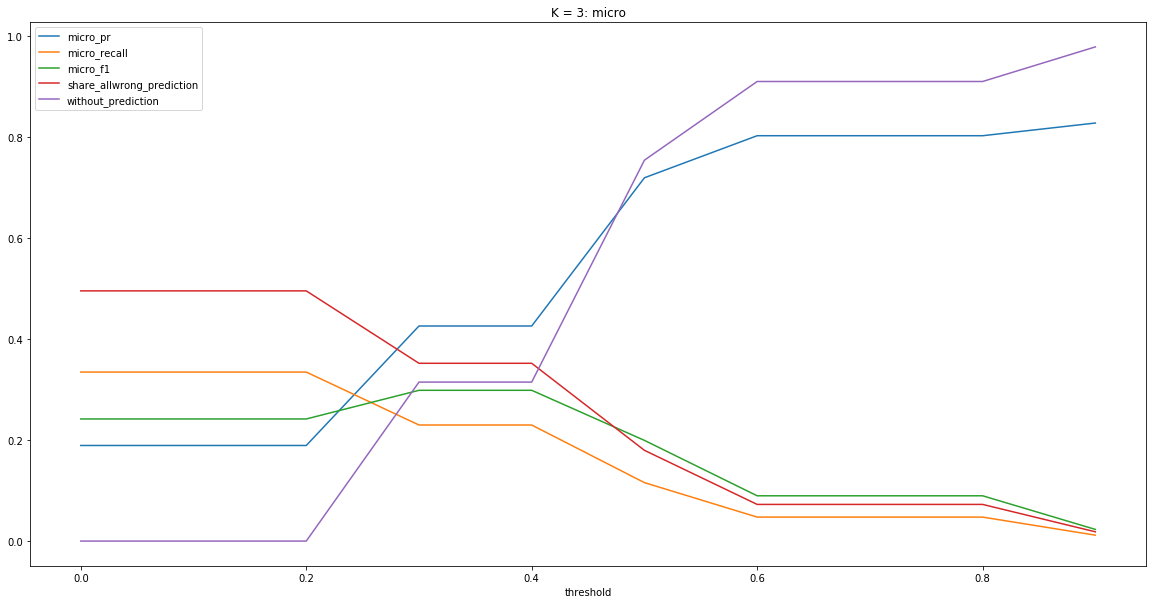
\includegraphics[width=0.49\textwidth]{figures/research-fields/random-forest-evaluation.png}\label{fig:rf}}
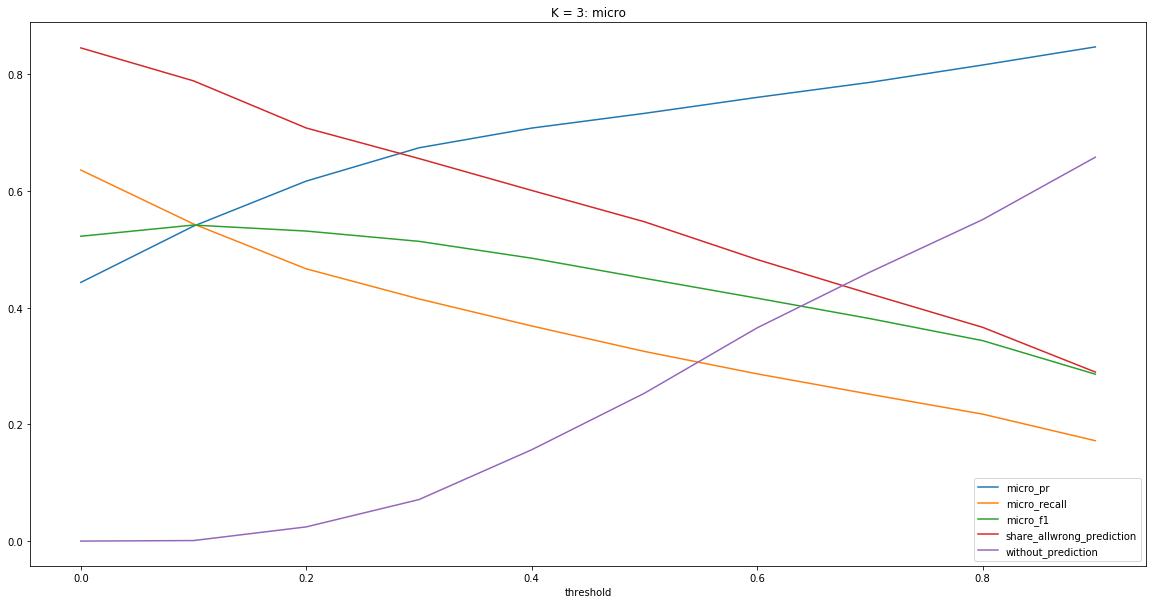
\includegraphics[width=0.49\textwidth]{figures/research-fields/fast-text-evaluation.png}
%\vspace{-1em}
\caption{Precision-Recall vs. Threshold}
\label{fig:results_fasttext}
\end{figure}



%The trends of micro f1, micro recall, and publications with just wrong predictions are falling smoothly, but the trend of micro precision and number of publications without any prediction are rising gradually. 
%The Micro precision still is higher than 0.7 for threshold 0.4. Also, the number of items without prediction is lower in threshold 0.4 than threshold 0.5 (the difference is about 0.1).

% We also experiment with random forest 



%purple curve (without_prediciton) 
%The measure without_prediction describes the share of publications without any prediction at all.
%E.g. if we only accept predicted labels with a model certainty of 60\%, 40\% of the publication have no predictions. 

%red curve (share_allwrong_prediction)
%The red curve describes the share of documents in the test set, which contain only wrong predictions for each threshold.
%This means when a threshold of 20\% certainty is selected 70\% of the publications have only wrong predictions. But if a threshold of 80\% certainty is selected only 40\% of the publications have only wrong predictions. 

    \section{Technical Documentation}
\label{sec:techdoc}
%(Documentation on how to install, train, configure, and run the model program)
The project contains the following modules listed in the order in which they are excecuted.

%=====================================================================================
%=====================================================================================
\subsection{Pre-processing}
%=====================================================================================
\subsubsection{PDF Text Extraction}
\textbf{Module name : }

Cermine_NlmJat_extractor\\
\textbf{Function: }

Converts each PDF files of a given folder to JATS XML Format. Each input PDF File is transformed to one XML File.\\
\textbf{Bash function call: }
\begin{lstlisting}
java -jar target/cermineXMLextraction-1.0.0-jar-with-dependencies.jar
\end{lstlisting}
\textbf{Parameter (2): }
\begin{lstlisting}
-s <source folder>\
-t <target folder>
\end{lstlisting}
\textbf{Returns: }

XML Files in JATS XML Format.\\
\textbf{Build: }

This is a Java program using Maven build tool.\\
\textbf{build call: }

mvn install

%=====================================================================================
\subsubsection{Extraction of text from JATS XML}
\textbf{Module name : }

preprocess-rcc-data\\
\textbf{Function: }

Transform text from JATX XML Format into a JSON File containing a list of textfields with essential metadata for each JATS XML file of a given folder.\\
\textbf{Bash function call: }
\begin{lstlisting}
`python3  ./jats_text_extractor.py `
\end{lstlisting}
\textbf{Parameter (4): }
\begin{lstlisting}
<source folder>
<target folder>
<limiting number of files to transform (-1: all)> 
<number of cores to use for multiprocessing (-1: all)>
\end{lstlisting}
\textbf{Returns: }

A JSON File for each given XML File in the source folder

%=====================================================================================
\subsubsection{Metadata Extraction}
\textbf{Module name : }

preprocess-rcc-data\\
\textbf{Function: }

Extracts structured metadata and references from all JATS XML files in a given folder into two Files.
One containing the metadata from all Publications in JATS XML files and one containing all references from the JATS XML Files.
The target file format is JSON.\\
\textbf{Bash function call: }
\begin{lstlisting}
python3  ./jats_metadata_extractor.py
\end{lstlisting}
\textbf{Parameter (3): }
\begin{lstlisting}
<source folder>
<target filename for metadata>
<target filename for references>
\end{lstlisting}
\textbf{Returns: }

Two JSON files containing metadata and references from all XML Files

%=====================================================================================
%=====================================================================================
\subsection{Dataset Mentions}
%=====================================================================================
\subsubsection{Dataset Mention Extraction}
\textbf{Module: }

dataset-mention-extraction\\
\textbf{Function:}

Extract dataset mentions from all JSON Files from a given folder with a given spacy model.\\
\textbf{Bash function call: }
\begin{lstlisting}
python3  ./predict_mentions.py
\end{lstlisting}
\textbf{Parameter (4): }
\begin{lstlisting}
<source folder>
<name of spacy model folder>
<target filename rcc-output>
<target filename internal format>
\end{lstlisting}
\textbf{Returns: }

Two JSON files containing the found dataset mentions in all given JSON Files.
One in RCC defined output.
One in Internal format including the senctence the dataset mention occures.\\
\textbf{Train: }

For training we submit a jupyter notebook with all needed code.
\emph{Train_spacy_ner_prod.ipynb}\\
\textbf{Build (For training only): }

Install english spacy language model.
This can be done with `python -m spacy download en`.

\begin{comment}
\textfg{}
For evaluation we first predict with the predictor which is used in production `predict_mentions.py`. We run this script on the test data and the result is a new field in paragraph data called `predicted_standoff`.
During evaluation with `evaluate.py` this filed is compared to the `standoff` field. The only parameter `evaluate.py` needs is the filename of the test data and the filename where the results should be saved in json format.
\end{comment}


%=====================================================================================
\subsubsection{Dataset Linking (only Phase 1)}
\textbf{Module: }

dataset-prediction\\
\textbf{Function: }

Links dataset mentions given a JSON file in internal format to datasets listed in a given JSON File.\\
\textbf{Bash function call:}
\begin{lstlisting}
python3  ./retrieve.py
\end{lstlisting}
\textbf{Parameter (3): }
\begin{lstlisting}
<JSON filename of extracted mentions>
<JSON filename of dataset list to match>
<output filename for dataset citations>
\end{lstlisting}
\textbf{Returns: }

JSON file in the format defined by the competition containing information about links between publications and datasets.

%=====================================================================================
%=====================================================================================
\subsection{Research Method Extraction}
\textbf{Module name : }

research-method-extractor\\
\textbf{Function: }

Extracts research method terms from JSON files with text information from publications.\\
\textbf{Bash function call: }
\begin{lstlisting}
java -jar target/gesisents-0.1-jar-with-dependencies.jar
\end{lstlisting}
\textbf{Parameter (3): }
\begin{lstlisting}
<source folder>
<target file name>
<Limit to reduce the number of processed files (-1:all)>
\end{lstlisting}
\textbf{Returns: }

A JSON file in the format defined by the competition containing information about publications and research methods.
\textbf{Build: }

This is a Java program using Maven build tool.\\
\textbf{build call: }

mvn install


%=====================================================================================
%=====================================================================================
\subsection{Research Field Classifier}
\textbf{Module name : }

research-field-detector\\
\textbf{Function: }

Classifies given abstracts with classoz Labels\\
\textbf{Bash function call: }
\begin{lstlisting}
python3  ./fasttext_predictor.py
\end{lstlisting}
\textbf{Parameter (4): }
\begin{lstlisting}
<filename of JSON file with abstracts>
<filename of fasttext model>
<filename of label dictionary in JSON>
<target filename labels in >
\end{lstlisting}
\textbf{Returns: }

A JSON file in the format defined by the competition containing information about publications and research fields.

\begin{comment}
#### 1. The classifier of FastText library (word embedding),
For training the fastText algorithm, the following code should be run:
```sh
python train_fastext_model.py
```
 In this code, for training the classifier, negative sampling 25 , epoch 150 , and ngram 2 are used as parameters. Also for applying the trained model on some test samples, the following script should be used:
 ```sh
python fasttext_predictor.py data_filename model_filename  label_dict  target
```
#### 2. Random forest algorithm from skilearn library
For training a random forest model, the following command can be used:
 ```sh
python train_sklearn_model.py
```
For training the classifier,  n_estimators=500, and random_state=42 are used as prameters. For applying the trained model on tes# Research Field Detector
t data, the following code should be use:
 ```sh
python sklearn_predictor.py
```
\subsubsection{SSOAR -- Metadata Harvestor}
For this reason a code is implemented to harvest metadata information. Here you can see how to run the harvestor 

code:
```sh
python harvest_ssoar.py
```
\subsubsection*{Evaluation}
For the evaluation, the following file can be used:
```sh
 ./evalouation_part/Evaluation_sklearn.ipynb
```
\end{comment}

    %\section{Unused stuff}







\begin{itemize}
    \item Problem: No ground truth
    \item Solution: Ground truth generation based on mention list and known datasets.
    \item Problem classes: Wrong annotatations (words are annotated as datasets, but the are not) and left out annotations (A dataset mention is not annoted with the procedure)
    \item Used model here?
\end{itemize}
\subsubsection{Mention lists as source}
\begin{itemize}
    \item Source of Information: Given mention lists from RCC
    \item benefits:
    \begin{itemize}
        \item Disambiguation Problem partly solved (Only mentions relevant for a concrete publication is mapped. Probability of Wrong annotation is low.
        \item Even vague mentions are annotated in this lists (Example: Monthly Statistics)
    \end{itemize}
    \item shortcomings:
    \begin{itemize}
        \item Left out Annotations: Only datasets with a known connection have mention lists; There are mentions of datasets which are not in the reference list)
        \item Definition of what is a dataset mention is not is interpreted differently by the annotator
        \item Because of the normalization of terms in the mention list some remappings might fail.
    \end{itemize}
    \item Used model here?
\end{itemize}

\subsubsection{Known dataset titles as source}
\begin{itemize}
    \item Problem: No ground truth
    \item Solution: Ground truth generation based on mention list and known datasets.
    \item Used model here?
\end{itemize}

\begin{itemize}
    \item Short Model description with Used Parameters
    \item Generation of training data in general
    \item What we did in phase 1 (Mapping from Mentionslist, including problems)
    \item What we did in phase 2 (Mapping from Dataset list, including problems)
    \begin{itemize}
        \item Goal better generalization
    \end{itemize}
    \item Eval First
    \item Eval second With qualitative results
\end{itemize}


We adopt a semi-supervised approach to address this task.
As a model for the NER task we used the standard NER-implementation of the NLP software library spacy\footnote{\url{spacy.io}}. The NER model 
The general idea to treat the lack of ground truth data is to use as much information about concrete mentions of datasets given by the RCC-team.

We treated the task of detecting dataset mentions in full texts as
For this, we trained a Named Entity Recognizer from [spacy](https://spacy.io/) a Natural Language Framework.

\subsubsection{Distant Supervision}
The challenge of missing ground truth data is the main problem to handle during this competition. Supervised learning methods to extract dataset mentions from text are not directly applicable for this reason.
As described in \ref{subsec:rcc-corpus} the corpus, the only information given about dataset mentions in text are a list of mentions for a part of the connections given in the first phase of the competition relating publications and datasets.
But not all connections of the training, evaluation and test set of the first phase of the competition contain this mention list.
Five percent of the connections in the train and development has no linked mentions in the mention list.
Unfortunately in the test set of Phase~1 which was made published for participants of Phase 2 only in 98\% of the connections an empty mention list is given.
Because of this there is no more potential training data for Phase~2.\\
                          (empty_share, #empty, #links)
    phase-1-develop                      (0.05, 5, 100)
    phase-1-test       (0.9800826756858324, 5216, 5322)
    phase-1-train      (0.05819239861793053, 320, 5499)
phase 2 Eval
\begin{enumerate}
    \item support 1983 mentions in 3018 publications from holdout set (20\%)
    \item 
\end{enumerate}
{'support': 1983,
 'partial_precision': 0.5124499141385231,
 'strict_precision': 0.4968517458500286,
 'partial_recall': 0.9029248613212305,
 'strict_recall': 0.875441250630358}

Examples of not in train ground truth 
________________________________
National Health and Nutrition Examination Surveys 17
1958 Philadelphia Birth Cohort Study 16
Patient’s and Physician’s Global Assessments 15
National Survey of Adolescents 12
Study of Women’s Health Across the Nation 10
First Austrian Dementia Report 9

\dots
National Household Transportation Survey 1
Iowa Transportation and Employment Survey 1
California’s Health Interview Survey 1
Annual Survey of Jails 1
National Household Survey of Drug Abuse 1
Arrestee Drug Abuse Monitoring researchers 1


Examples in groundtruth of train
________________________________
National Health and Nutrition Examination Survey 137
Third National Health and Nutrition Examination Survey 97
National Longitudinal Study of Adolescent Health 87
Health and Retirement Study 53
National Crime Victimization Survey 39
Current Population Survey 36
\dots
1984 National Health Interview Survey 1
2000 Census of State and Federal Adult Correctional Facilities 1
1976 Detroit Area Study 1
Epidemiologic Catchment Area Program 1
= National Social Life, Health, and Aging Project 1
U.S. Health and Nutrition Examination Survey 1



Even though our approach uses supervised machine learning, to handle the lack of a ground truth we use  training data generated with help of the aforementioned mention lists in the first phase. 
The result is a weakly labeled training corpus. This method is inspired by \cite{lee2016bagging}. The concrete realisation is described in \ref{subsec:ground-truth-phase1}.\\
\sd{could you state some more details here about the scale and quality of the labels (or the limitations)?}
For the second phase we are facing the following challenges.
\sd{start this with a more general statement about "lack generalisability of the selected ground truth" which seems to be the main point.}
\sd{sentence below refers to your weakly labeled training data? with "publications of second phase" you mean the test/evaluation set?}
At least half of the publication of the first phase was selected because of known relations to datasets in the ICPSR dataset list.
However, only around 5,000 of the 10,000 dataset records were used in the training set.
The publications of the second phase were selected randomly from a social science corpus of sage publication as described in \ref{subsec:rcc-corpus}.
\sd{statement below: isn't it causal, i.e. "the publications containing ICPSR are expected to be low, therefore the model will not perform/generalise well"}
So we expect not only the publication containing datasets from the ICPSR dataset records lower, but also the model trained on mentions of around 500 of them not to generalize well on the new corpus.
How we generated a weakly annotated corpus as training corpus for Phase 2 we describe in \ref{subsec:ground-truth-phase2}.



\subsubsection{Ground truth Generation Phase 1}
\label{subsec:ground-truth-phase1}
\sd{I'd merge this into the section above for the sake of readability and go step by step.}
As training data we used remapped mentions from the data\_set\_citation.json files mentions\_lists.

 
\subsubsection{Ground truth Generation Phase 2}
\label{subsec:ground-truth-phase2}
 
\subsection{Evaluation}
%\subsubsection{Metrics}
\subsubsection{Evaluation Phase 1}

\subsubsection{Evaluation Phase 2}


\begin{comment}
The used software components are:
\begin{itemize}
    \item Preprocessing
        \begin{itemize}
            \item PDF extraction: \emph{Cermine\_NlmJat\_extractor}
            \item Metadata extraction and preprocessing:\\ \emph{preprocess-rcc-data}
        \end{itemize}
    \item Dataset Linking
        \begin{itemize}
            \item Find data set mentions: \emph{dataset-mention-extraction}
            \item Predict citations: \emph{dataset-prediction}
        \end{itemize}
    \item Research Field Classification
        \begin{itemize}
            \item Identify research fields: \emph{research-field-detector}
        \end{itemize}
    \item Research Methods Extraction
        \begin{itemize}
            \item Find research methods in a text:\\ \emph{research-method-extractor}
        \end{itemize}

\end{itemize}
\end{comment}


    \phantomsection
\subsection{Acknowledgments} 
\addcontentsline{toc}{section}{Acknowledgments}
We would like to thank GESIS for giving us the time and resources to participate in the competition.
%\phantomsection
\subsection{References} 
\bibliographystyle{unsrt}
\bibliography{bibliography}

\end{document}


%% 
%% Review of white paper
%% o   Clear overview of tasks
%% o   Solid presentation of approach
%% o   Major advantage given their local dataset:  Social Science Open Access Repository %% (SSOAR) – but use what you have is a GREAT principle.
%% o   Professional effort!!!  -- Approach, documentation, & justification.
%% o   Problem:  quality of their results, lower than others.

% all
% ------
%•	In both field and dataset classification, what types of errors did you get? Were these the type of errors you would expect or were there strange ones? Are your errors coming from contextual features or from noun phrase features?

%% Todos:
% research methods:
% ----------------
%"I would have liked to have seen a little more information on the shape features"

% research fields:
% ----------------
% "why did you choose 44 fields"
% More about source of classification
% "•	If, instead of abstracts, you train on summarizations, how do you think it will affect your results?"

% datasets:
%•	You may want to consider looking into the area called ‘weak supervision’. Specifically, you mentioned that some of the things that spaCy model was returning looked good, and you could add those in as an additional training data - other terms for that could be ‘co-training’ or ‘bootstrapping’.
% No. weak supervision

% Words about matching (citation?) •	You said that the mentions problem was more interesting to confront than citations - do you have any thoughts on why you performed worse on the citation problem than on the mentions?

